% LaTeX layout by Jonas Kahler, jonas@derkahler.de
% HashTux SAD Document
% Group Tux:
% Aman Dirar, Jerker Ersare, Jonas Kahler, Dennis Karlberg
% Niklas le Comte, Marco Trifance, Ivo Vryashkov
% Chapter 2 - Architectural Drivers
\label{ad}
\chapter{Architectural Drivers}

%% Functional Reqs
\section{Functional Requirements}
{\tabulinesep=1.4mm
\begin{tabu}{|l|l|}
\hline
\taburowcolors{gray!25..white}
\multicolumn{2}{|l|}{Must} \\
\hline
\taburowcolors{}
FR1 & \parbox[t]{105mm}{The user must be able to search for a term and get
   matching results in the form of multimedia content from social media services
   (initially we focus on Twitter, Instagram and Youtube). The way in which the
   content is displayed must conform to the terms and conditions for each social
   media API respectively.} \\
\hline
FR2 & \parbox[t]{105mm}{The user must be able to select different options when
   searching for a term. Options are which services to search for (eg only
   twitter), content type (eg only images and videos), languages (eg only
   french).} \\
\hline
FR3 & \parbox[t]{105mm}{The user must be able to select different options for
   how the content is displayed, such as tile size for displayed results
   (eg small) and refresh rate for updating the grid (eg fast).} \\
\hline
FR4 & \parbox[t]{105mm}{The user can`freeze'' (and then `unfreeze'') a certain
   media item (tile in the grid), which means it will not be swapped out for a
   more recent media item in subsequent updates while it is `frozen''.} \\
\hline
FR5 & \parbox[t]{105mm}{The user must be able to search for content that is
   non-recent, for example content from two days ago.} \\
\hline
FR6 & \parbox[t]{105mm}{The client UI must provide the user with the option of
   buying a license for commercial use. All users should also be able to donate
   money to our project through PayPal.} \\
\hline
FR7 & \parbox[t]{105mm}{The client UI must be optimized for full-screen view and
   continue to show content if left unattended for an extended period of
   time.} \\
\hline
\end{tabu}} \\ \\
%%%%% New page %%%%%
{\tabulinesep=1.4mm
\begin{tabu}{|l|l|}
\hline
\taburowcolors{gray!25..white}
\multicolumn{2}{|l|}{Should} \\
\hline
\taburowcolors {}
FR8 & \parbox[t]{108mm}{The user should be able to see different user habit
   statistics in a separate part of the client UI. Dimensions: at least search
   terms, web browsers and platforms (operating systems) and their respective
   popularity among HashTux users.} \\
\hline
FR9 & \parbox[t]{108mm}{The user should be able to view different periods of the
   user habit statistics dimensions.} \\
\hline
FR10 & \parbox[t]{108mm}{The user should be able to search (free-text) in the
   statistics part of the client UI for keywords in each dimension.} \\
\hline
\taburowcolors{gray!25..white}
\multicolumn{2}{|l|}{Could}  \\
\hline
\taburowcolors{}
FR11 & \parbox[t]{108mm}{On the front page or wherever appropriate, the user
   should be able to see current trends in social media and in the search habits
   of users to get some inspiration on what to search for.} \\
\hline
\taburowcolors{gray!25..white}
\multicolumn{2}{|l|}{Wont}   \\
\hline
\taburowcolors{}
FR12 & \parbox[t]{108mm}{The user should be able to chat with other users of the
   application.} \\
\hline
\end{tabu}}

%% Quality Reqs and Secenario Analysis
\section{Quality Requirements and Scenario Analysis}
Quality requirements for our project in order of significance (most important
first). Quality scenarios are provided for each quality attribute as well as a
brief description. For tactics addressing the QA mentioned, see
\hyperlink{tactics}{Tactics}.

%%% Availability
\subsection{Availability}
Our goal for the product is to have an uptime of 99.999\%. This value is
expected when running the full server-side component stack on 3 servers or more.
For a lower number of servers running the stack, we expect an uptime of the
system of 99\%.
\begin{figure}[ht]
  \centering
  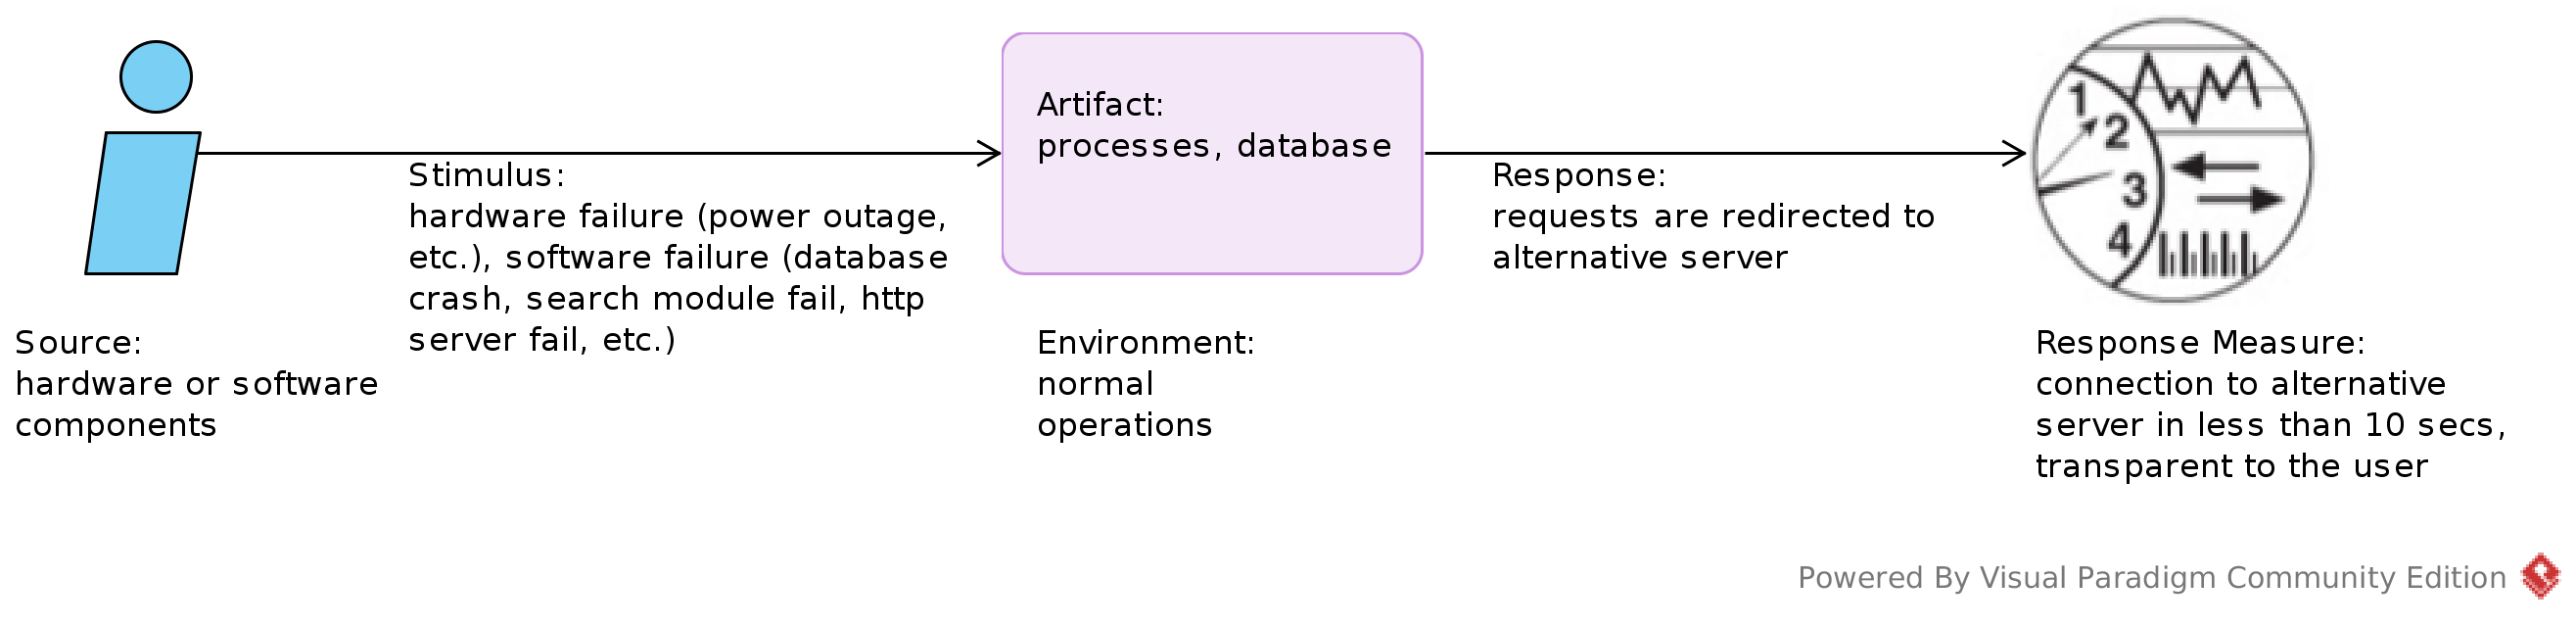
\includegraphics[width=1\textwidth]{availability_scenario.png}
  \caption{Availabilty Scenerio}
\end{figure}

%%% Performance
\subsection{Performance}
The system needs to respond quickly enough for the user not to be discouraged
from using our product. On average requests should be processed in less than
5sec. Database operations should be performed, on average, in less than 1sec.
\begin{figure}[ht]
  \centering
  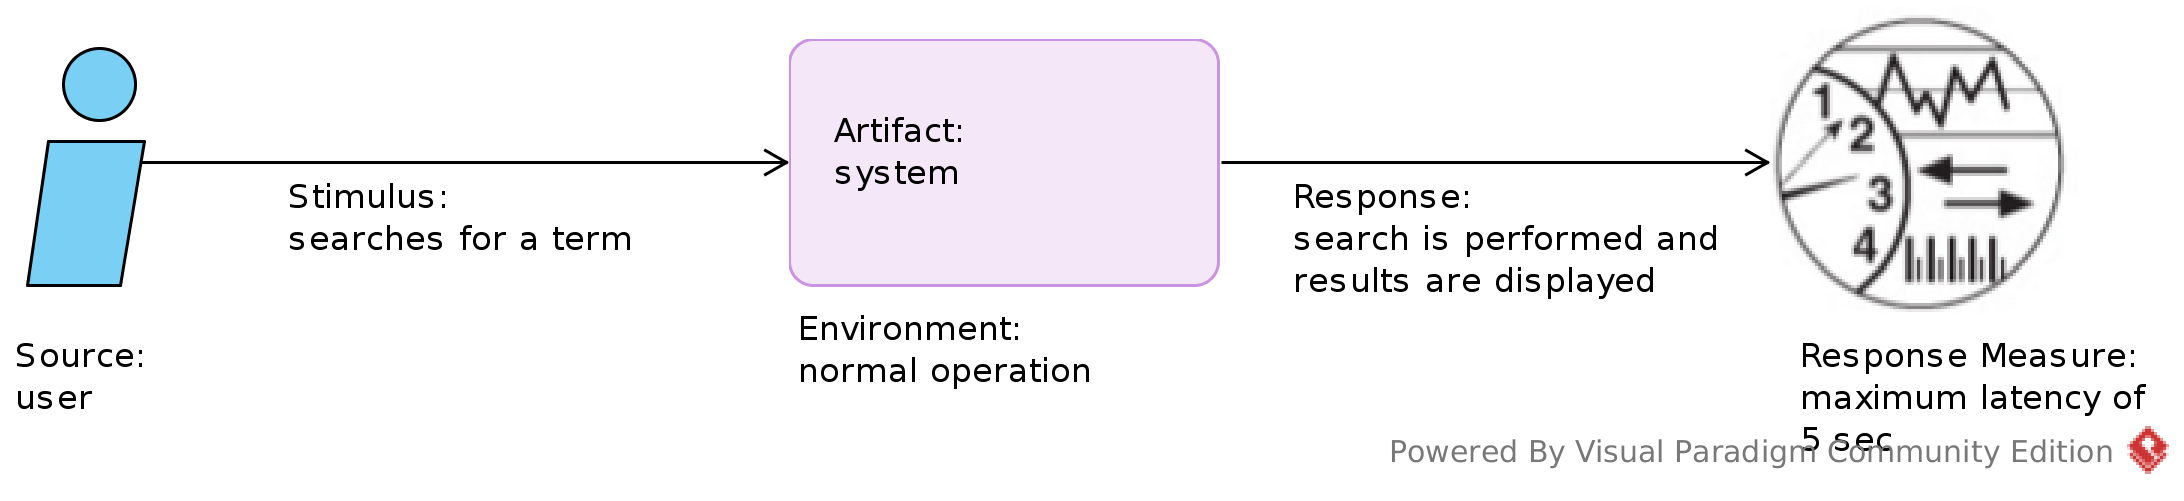
\includegraphics[width=1\textwidth]{performance_scenario.png}
  \caption{Performance Scenerio}
\end{figure}

%%% Modifiabilty
\subsection{Modifiability}
The system should be designed to support easy modification. This requires aiming
for having loosely coupled modules and a clear separation of concerns. For
example, adding new modules to support different social media services should
require low effort from the development team.
\begin{figure}[ht]
  \centering
  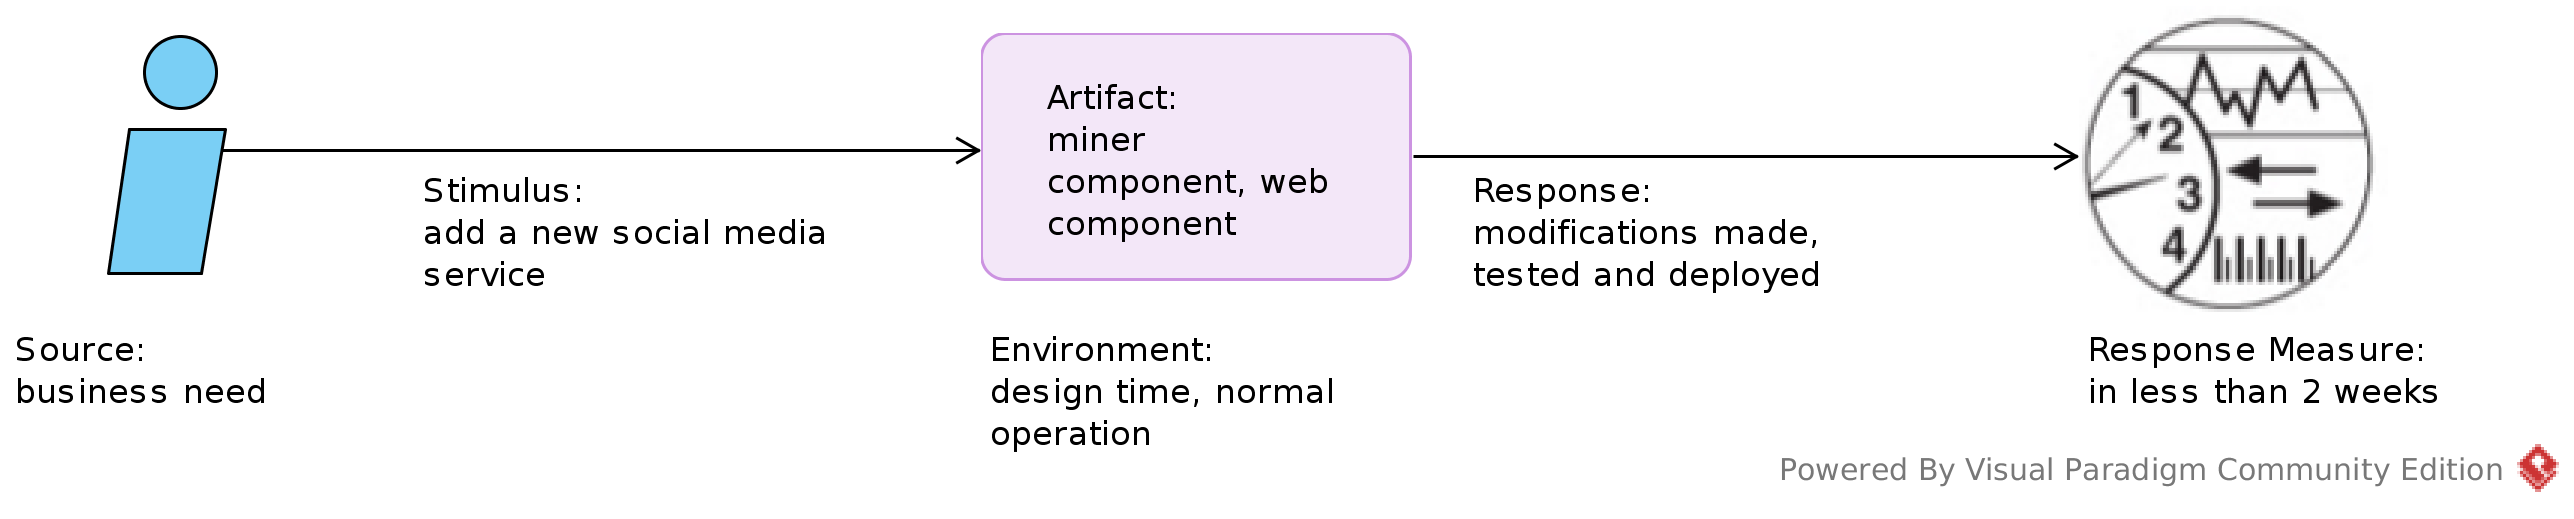
\includegraphics[width=1\textwidth]{modifiability_scenario.png}
  \caption{Modifiability Scenerio}
\end{figure}

\newpage

%%% Usability
\subsection{Usability}
The system should be easy to use in an intuitive way. This is hard to quantify,
but we want our application to be as easy to use as the social media services we
get content from, i.e. the typical user shouldn't have to consult a user manual
to understand the provided features and options.
\begin{figure}[ht]
  \centering
  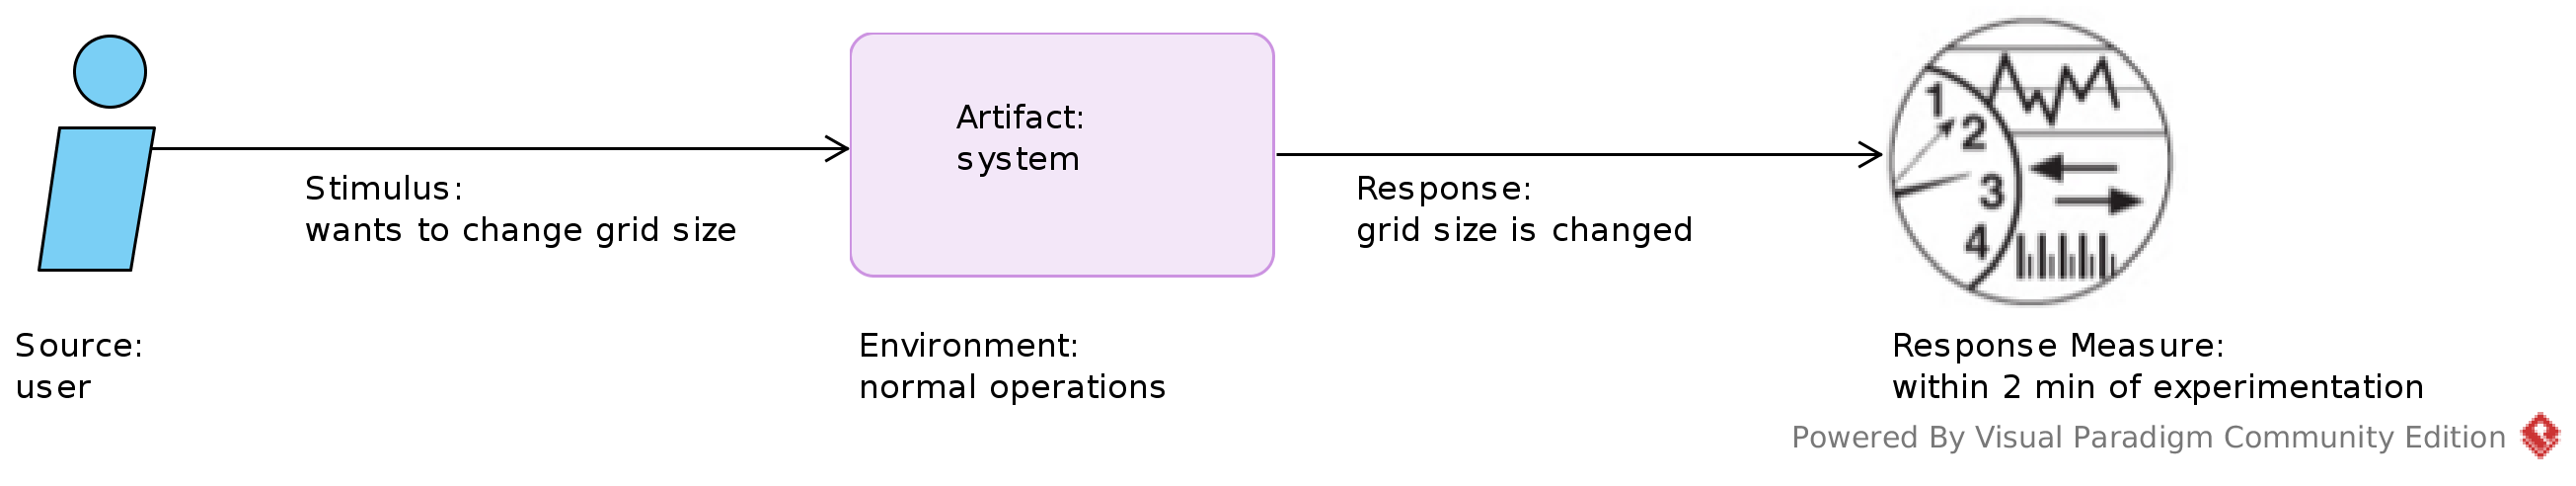
\includegraphics[width=1\textwidth]{usability_scenario.png}
  \caption{Usability Scenerio}
\end{figure}

%%% Security
\subsection{Security}
The system should have security mechanisms to prevent DDoS attacks and
unauthorised access to our databases. Security is not our primary concern
because we do not store or deal in any way with sensitive data like user login
credentials or bank accounts. However, to guarantee availability, we must aim to
minimize security vulnerabilities, both when designing, implementing and
deploying our system.
\begin{figure}[ht]
  \centering
  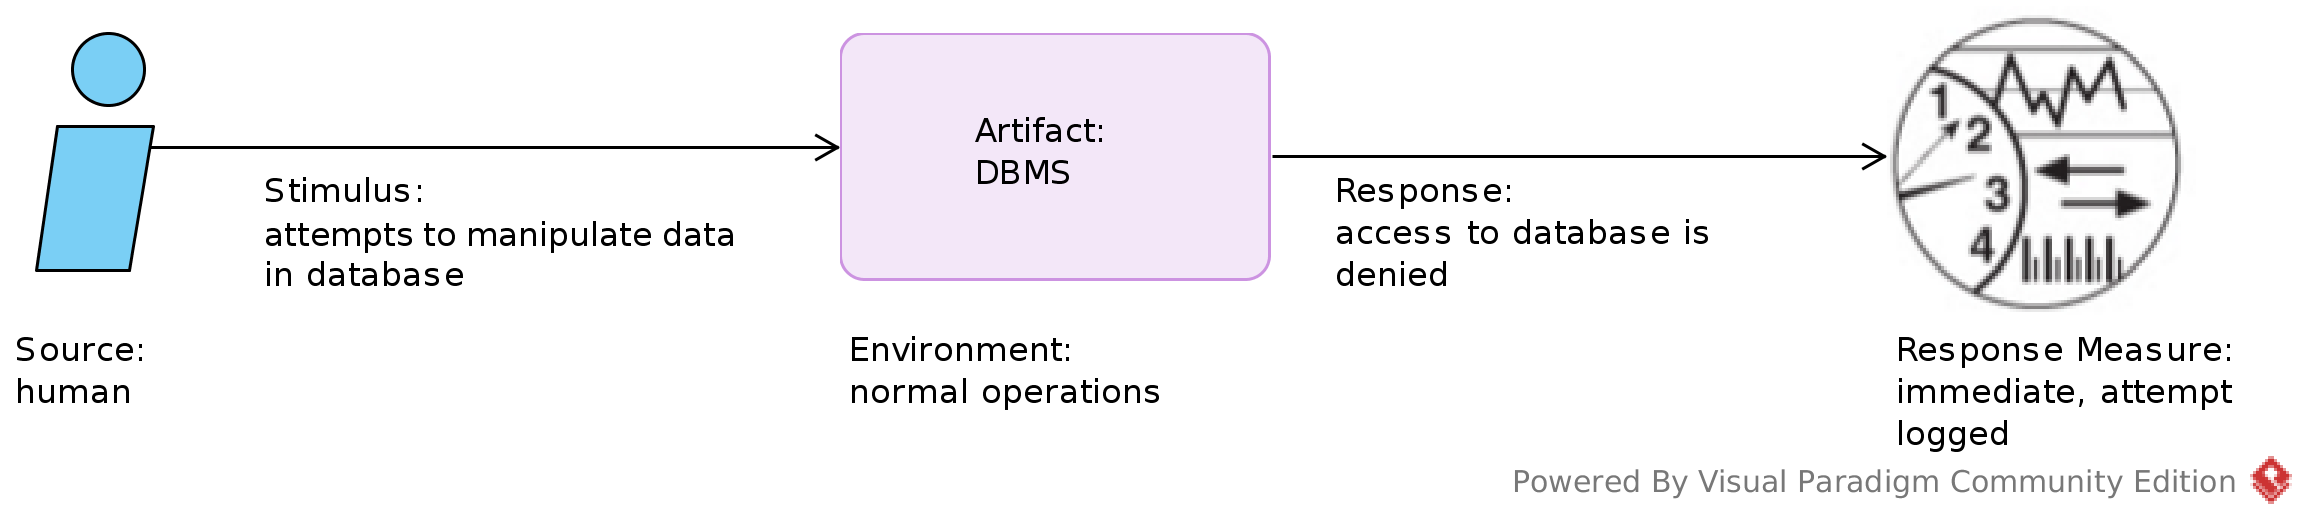
\includegraphics[width=1\textwidth]{security_scenario.png}
  \caption{Usability Scenerio}
\end{figure}

%% Utility Tree
\section{Utility Tree (Tabular Form)}
{\tabulinesep=1.4mm
\begin{tabu}{|c|c|c|c|}
\hline
\taburowcolors{gray!25..white}
\parbox[t]{2cm}{\textbf{Quality \\ Attribute}}
   & \parbox[t]{25mm}{\textbf{Attribute \\ Refinement}}
   & \parbox[t]{5cm}{\textbf{ASR}}
   & \parbox[t]{12mm}{\textbf{Impact}} \\
\hline
\taburowcolors{}
\multirow{2}{*}{\parbox[t]{2cm}{Availability}}
   & \multirow{2}{*}{\parbox[t]{25mm}{H/W or S/W failure}}
      & \parbox[t]{5cm}{Power outage: requests are redirected to an alternative
         server in less than 10 sec}
      &  \parbox[t]{12mm}{(H, M)} \\ \cline{3-4}
   &  & \parbox[t]{5cm}{Database failure: module responsible for database
         operations is reconfigured to use an alternative database in less
         than 3 sec}
      & \parbox[t]{12mm}{(H, M)} \\
\hline
\multirow{2}{*}{\parbox[t]{2cm}{Performance}}
   & \parbox[t]{25mm}{Perform search}
      & \parbox[t]{5cm}{Search is performed and results are displayed in less
         than 5 sec}
      & \parbox[t]{12mm}{(M, M)} \\ \cline{2-4}
      & \parbox[t]{25mm}{Check \\ statistics}
      & \parbox[t]{5cm}{Statistics are fetched from database and displayed in
         less than 5 sec}
      & \parbox[t]{12mm}{(M, M)} \\
\hline
\parbox[t]{2cm}{Modifiability}
   & \parbox[t]{25mm}{Add new social media service}
   & \parbox[t]{5cm}{Integrate a new social media service in less than 2 weeks
      (80 man-hours)}
   & \parbox[t]{12mm}{(M, M)} \\
\hline
\parbox[t]{2cm}{Usability}
   & \parbox[t]{25mm}{User wants to change grid size}
   & \parbox[t]{5cm}{The grid size is changed within 2 min of experimentation}
   & \parbox[t]{12mm}{(M, L)} \\
\hline
\parbox[t]{2cm}{Security}
   & \parbox[t]{25mm}{Database integrity}
   & \parbox[t]{5cm}{Unauthorised access to the database is denied}
   & \parbox[t]{12mm}{(L, L)} \\
\hline
\end{tabu}}

%%%%% Page break %%%%%
\newpage

%% Tactics
\hypertarget{tactics}{
\section{Tactics - Risks, Tradeoffs and Sensitivity Points}}
The tactics applied to achieve the above mentioned quality attributes are
elaborated here and some risks, tradeoffs and sensitivity points are discussed.

\subsection{Availability}
\textbf{Timeout} - this tactic is used to detect if the backend server is
available to serve requests. If the time exceeds the configured value, the web
application tries to connect to an alternative backend server. This helps to
ensure that each instance of our PHP application can establish a connection with
an available backend server. \newline
A tradeoff for this tactic is a certain latency in responding to a search
request when the currently preferred backend server goes down
(see Reconfiguration for how we handle this). \\ \\
\textbf{Active Redundancy} - for our application we have servers standing by
(up and running live) and waiting to serve requests at any time. This also
ensures the mentioned uptime of the system. \\ \\
\textbf{State Resynchronisation} - used to provide a synchronised state of the
collected user habit data across all available databases. This process takes
place every minute. \\ \\
\textbf{Reconfiguration} - we use this in two areas:
\begin{itemize}
  \item We use this tactic to maintain availability when writing and reading to
     the database. If at any point the current database used for operations goes
     down, the module responsible for database procedures is reconfigured to use
     an alternative database.
  \item When a backend server fails to respond to a request in time, it will be
     marked in the web applicationâs list of servers as down (with a timestamp
     of the incident). The web application will re-evaluate which backend server
     to connect to, and remember this decision. After a certain configurable
     time period, the incident will be âforgottenâ, so that the original server
     may be brought back to service (provided that it is now responding).
\end{itemize}

%%% Performance
\subsection{Performance}
\textbf{Limit Event Responses} - this tactic is used when handling requests in
the backend server to provide the required performance rates. This tactic is
used together with the \textit{Bound Queue Sizes} tactic. For our miner server,
which is responsible for spawning workers to process requests, we have a queue
size limit set to 1000. If the limit has been reached and the current request
cannot be processed, the miner server sends a message back to the PHP
application to notify it that there are currently too many requests served
and an alternative server should be tried. \\ \\
\textbf{Introduce Concurrency} - a key tactic used in our system. It helps for
parallel execution of operations and reduces the overall latency of serving
requests. Concurrency is used in the backend server for managing clients, i.e.
new threads are created for each request. Each request to the social media APIs
are also handled in parallel. The same goes for database operations. \newline
A risk of race condition when using concurrency is possible. This can occur
especially when reducing the re-reduced results for caching the user statistics.
Therefore, we created a custom pmap function that avoids these race conditions.
\\ \\
\textbf{MapReduce} - this tactic is used when caching summarizations of various
user statistics for our statistics page. The user habits we collect generate a
large amount of data and the use of MapReduce helps with precaching the
statistics. The cached data is generated and stored in a separate database every
hour and can then be quickly fetched when the client UI needs to display it.

%%% Modifiability
\subsection{Modifiability}
A risk in general for modifiability is increased overhead when using
intermediaries. This can affect the overall performance of the system. We do not
identify this to be an issue for our product as it is. However, if the
application is to be developed further and the size and scope increases, a
tactic like \textit{Reduce Overhead} should be considered to maintain the agreed
performance levels. \\ \\
\textbf{Increase Semantic Coherence} - this tactic addresses the separation of
concerns. Each module has a clear responsibility and reduces the likelihood of
side effects and errors when making changes. \\ \\
\textbf{Restrict Dependencies} - this tactic addresses the concept of coupling
between modules. Each module can interact with a certain number of other modules
and low dependencies result in low cost and effort when implementing a change.
It also keeps the complexity level low.

%%% Usability
\subsection{Usability}
\textbf{Aggregate} - the different options for our application are presented in
one simple view. This allows easy accessibility (all options are aggregated in
one place) and reduced time in changing them (no need for the user to search for
multiple menus containing different alternatives).

%%% Security
\subsection{Security}
\textbf{Authenticate Actors} - default security mechanism provided by the DBMS.
\\ \\
\textbf{Change Default Settings} - during deployment, we do not use the default
settings that come with the different services in use. For example, CouchDB
listens by default on port 5984 which we changed. \\ \\
\textbf{Firewall} - from a deployment point of view, we see it as natural to
use firewalls on each server.

%% Constraints
\section{Constraints}

%%% Overall Contstraints
\subsection {Overall Constraints}
According to the assignment definition, our application needs to\dots
\begin{itemize}
  \item be distributed.
  \item consist of at least three tiers.
\end{itemize}
We were also encouraged to use a non-relational database management system.
\newline
All of the above affect the architecture significantly. So does the following
details of our product vision:
\begin{itemize}
   \item Our product is a web application, intended to be accessed via a web
    browser. The product should be optimized for full-screen display of content.
\end{itemize}

%% API Limitations
\hypertarget{apilimits}{
\section{API Limitations}}
Requests to Instagram, Twitter and Youtube Data APIs represent a central part in
most of the use cases described in this document. However, APIs impose rules and
limitations on how to use and render the retrieved data on third-party
applications. You can find a list of references to the relevant documents in
\hyperlink{refapis}{Appendix}. \newline
Although these rules are mandatory and cannot be ignored, they do not seem to
affect the architecture of the system as a whole. For this reason we decided to
discuss this aspect of the implementation separately from the architectural
drivers described in the previous section. In this section we briefly discuss
the limitations that have been considered relevant in the planning phase and the
solutions we undertook during implementation.

%%% Display Requirements
\subsection{Display Requirements}
\subsubsection{Instagram}
No limitations imposed by Instagram regarding displaying of content.
\subsubsection{Twitter}
\underline{Limitation}: Tweets rendered in third-party web applications must
comply with the Twitter Display Requirements. In details, Twitter identifies a
minimum set of items (such as date, text, profile picture\dots) that must be
displayed and sets some rules on the positions and links provided by these
items. \newline
\underline{Solution}: The use of embedded tweets ensures compliance with the
display requirements discussed above. However, being our application focused
primarily on the media content of retrieved feeds, we opted for a new display
format that is fairly homogeneous among feeds coming from different
social-medias. Moreover, the use of embedded tweets is limited to 10 million
tweets per-day. Although the limit seems to be fairly high for our application,
the choice of rendering tweet objects in our own format makes \textit{HashTux}
not subject to this kind of limitation.
\subsubsection{YouTube}
\underline{Limitation}: \textit{``[\dots] any YouTube logo used within an
application must link back to YouTube content or to a YouTube component of
that application.''} \newline
\underline{Solution}: We decided not to use any logo or trademark for rendered
YouTube feeds.

%%% Search Limitations
\subsection{Search Limitations}
\subsubsection{Instagram}
\underline{Limitation}: Unfortunately, Instagram does not provide a proper
search service for non-recent posts (e.g. posts from 3, 4 or more days ago).
They make use of pagination and each results page has a unique id that can be
used later to retrieve results before or after a certain page id. The problem is
that they have no connection between page id and the timeframe that this page
represents. For example, if we want to fetch content posted 2 days ago, there is
no way to obtain the page that holds results for that time period to display
when a history search is performed. \newline
\underline{Solution}: We decided to exclude Instagram from the history search
function. For now we search only Twitter and YouTube for non-recent content.

%%% Confidentiality Limitations
\subsection{Confidentiality Limitations}
API Authorization Keys for all the involved APIs are subject to security rules.
API Keys for \textit{HashTux} are stored on our servers and are not accessible
from outside.

%%% Privacy
\subsection{Privacy}
The content retrieved and displayed on our web page is flagged as “public” and
fulfills the privacy requirements specified in the the APIs Terms of Use
(see \hyperlink{refapis}{Appendix}).